\paragraphn{Quantitative analysis 1 - Clause weights}
The performance in terms of \textit{macro f1 examples} obtained by varying the initial clause weights is available in Figure~\ref{fig:wandb_weights_comparison}. Looking at the graphs, we can observe a common behavior: regardless of the KB mode, the influence of different weights is visible only in the first 15-20 epochs (i.e., the red line in the graph is above the others in the initial epochs). Especially for the Hybrid mode, we can see in Figure~\ref{fig:wandb_weights_comparison_h} how the largest weight gives a clear initial boost to the performance. However, the boost tends to diminish over the epochs until it disappears. Another interesting behavior can be found in Figure~\ref{fig:wandb_weights_avg_pred_start}, which shows the evolution of the \textit{average predictions number} in the first 20 epochs. From the figures, we can observe that the larger the weight, the higher the number of predictions, and the larger the weight, the higher the performance. We can deduce from these results that the increased performance is due to an increased number of correct predictions, otherwise we would not see an increment in the performance. To conclude, we can say that a major influence of KENN helps the network to learn faster when it has not yet seen a big amount of training examples.
\\\\
\textit{\textbf{Note:} the previous considerations still apply to the other metrics not reported here}

\begin{figure}
     \centering
     \begin{subfigure}{0.8\textwidth}
         \centering
         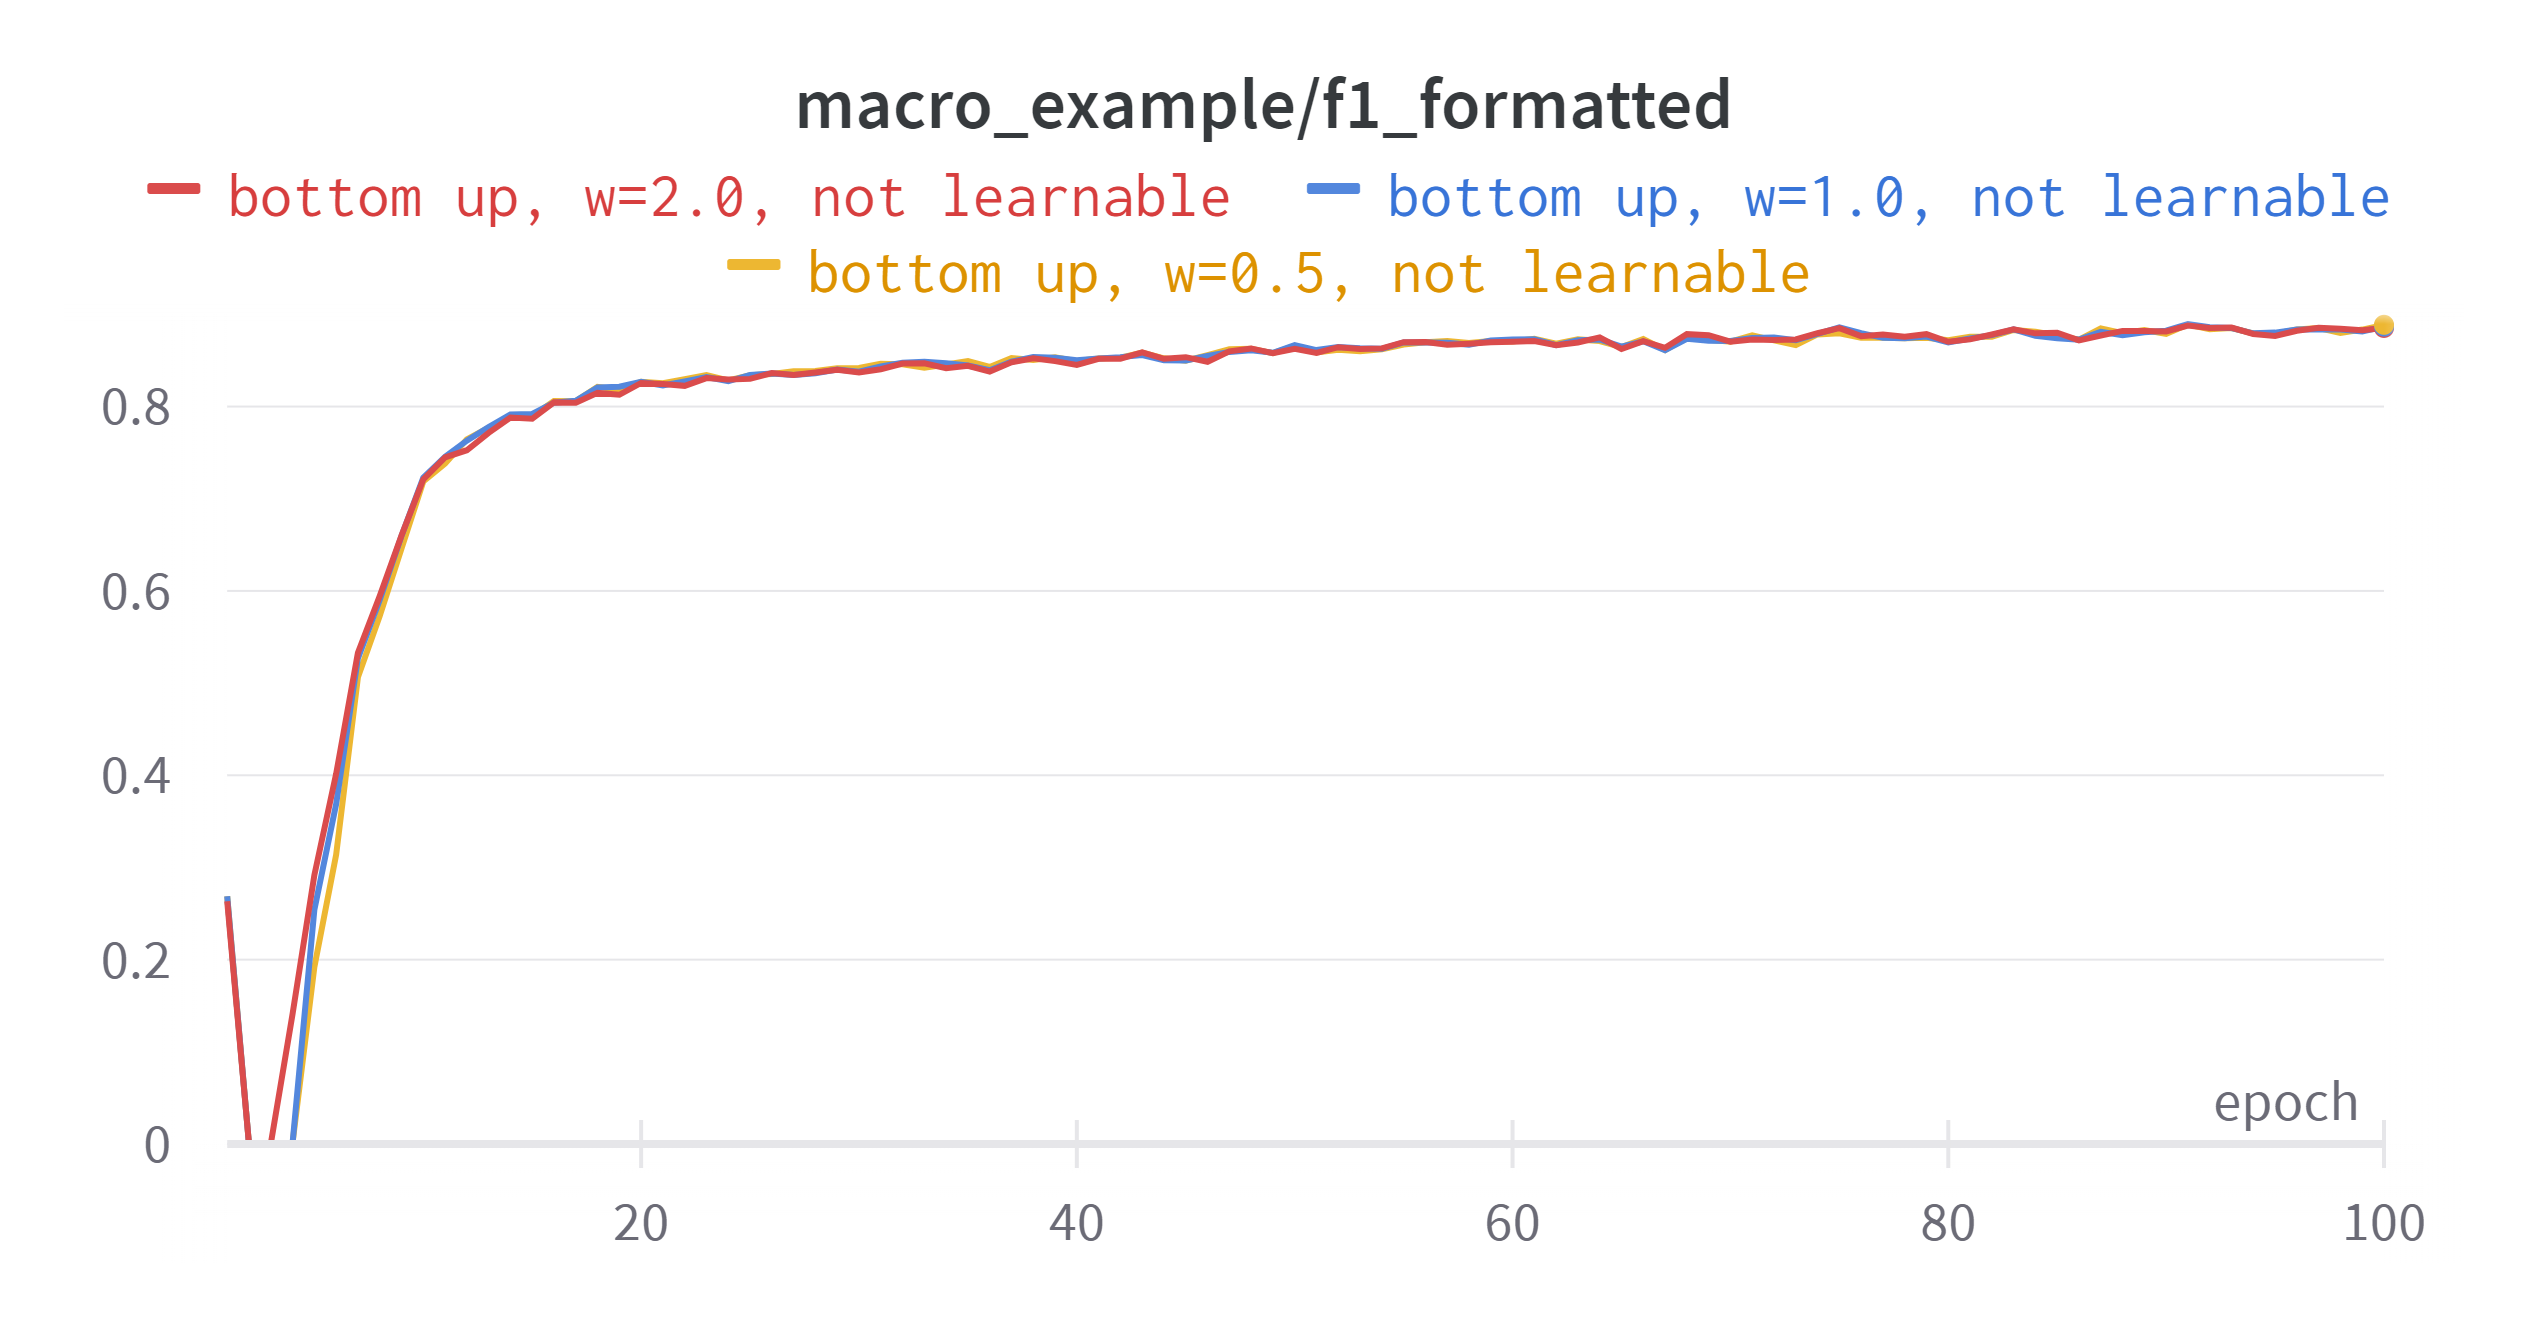
\includegraphics[width=\textwidth]{figures/wandb_weights_bottom_up_macro_ex_f1.png}
         \caption{Bottom Up}
     \end{subfigure}
     \vfill
     \begin{subfigure}{0.8\textwidth}
         \centering
         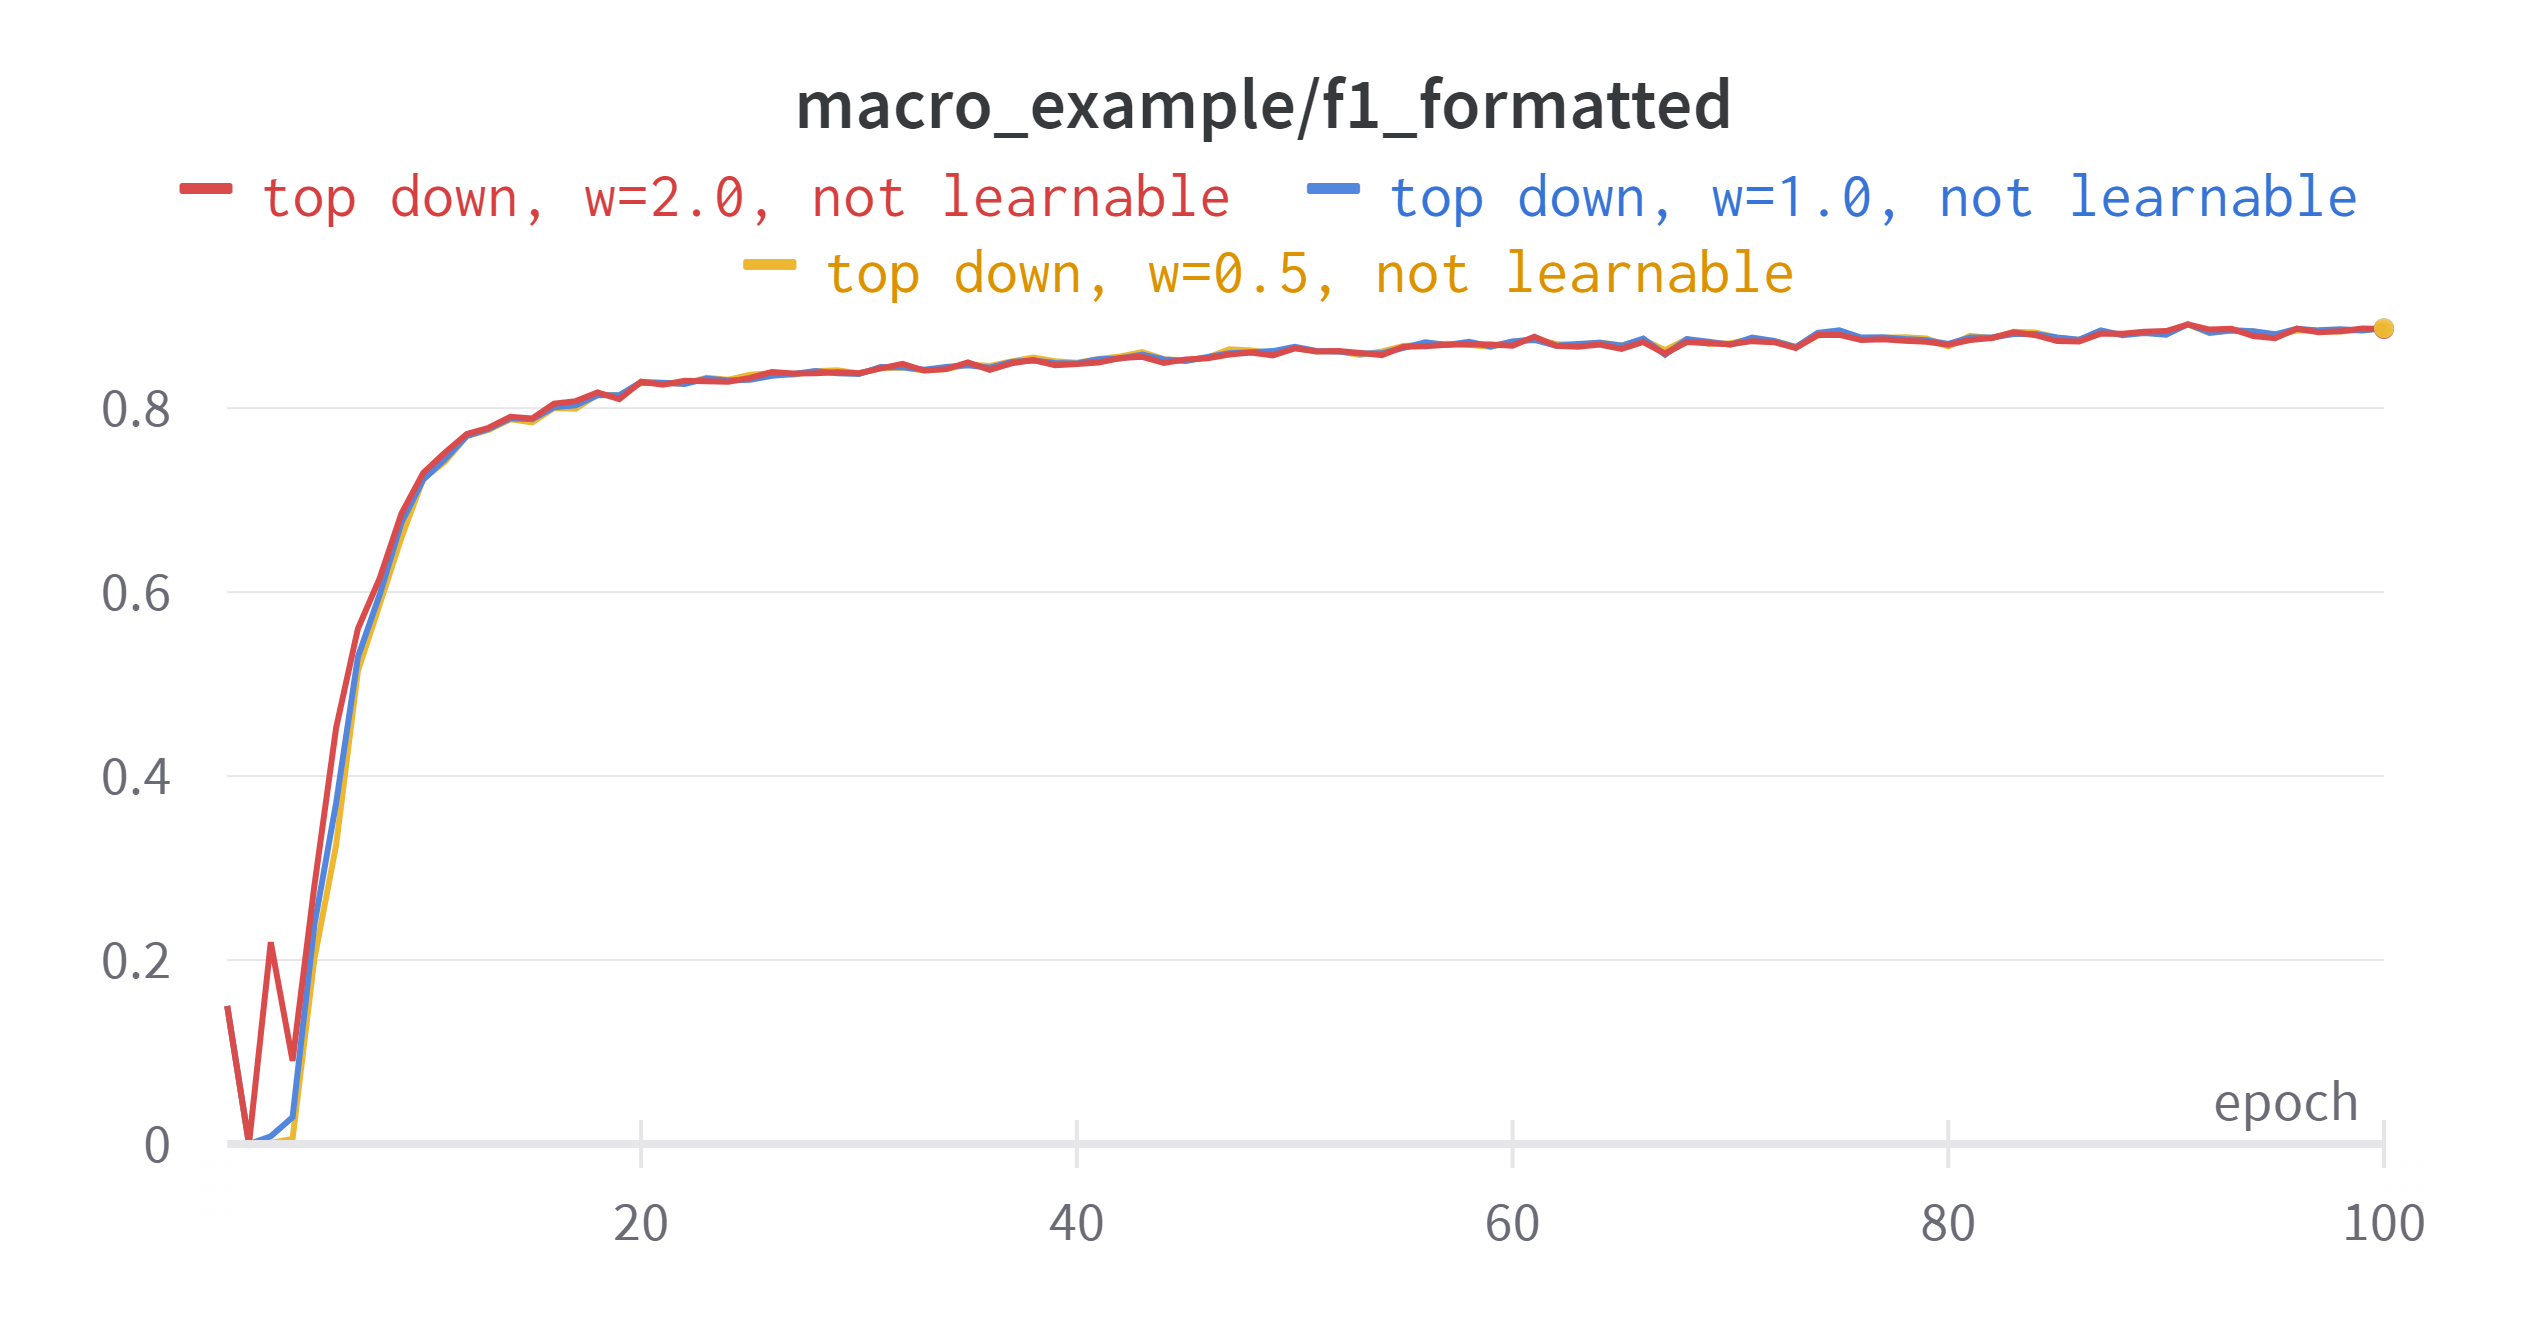
\includegraphics[width=\textwidth]{figures/wandb_weights_top_down_macro_ex_f1.png}
         \caption{Top Down}
     \end{subfigure}
     \vfill
     \begin{subfigure}{0.8\textwidth}
         \centering
         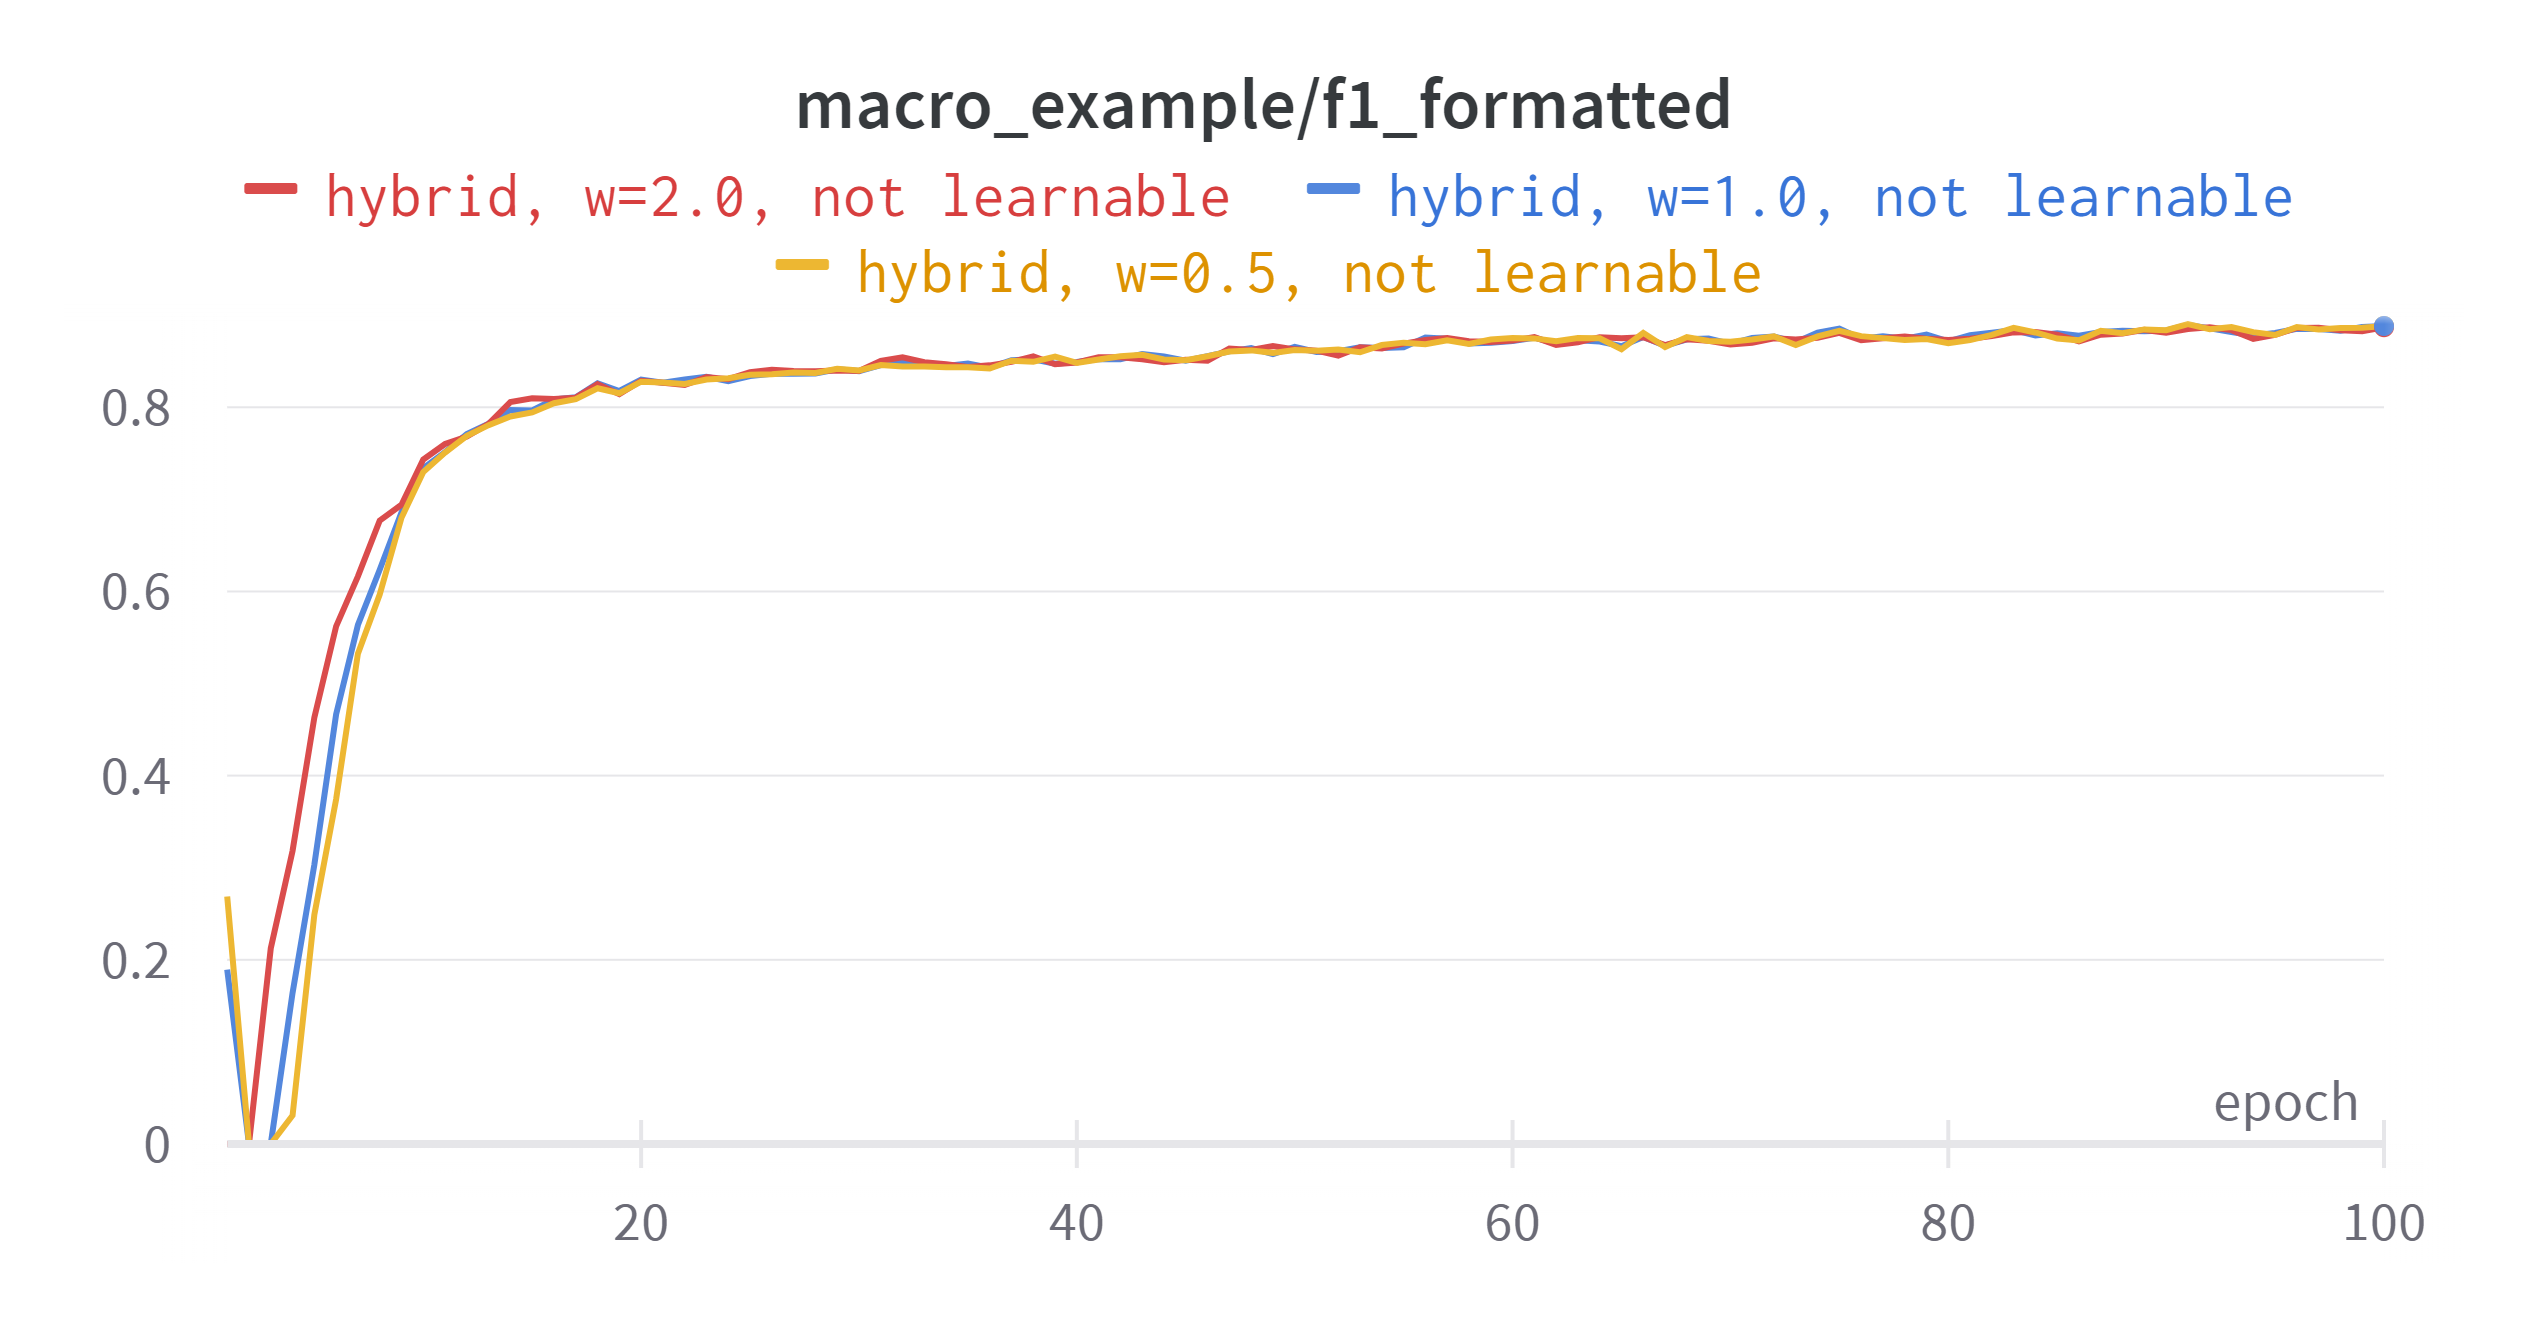
\includegraphics[width=\textwidth]{figures/wandb_weights_hybrid_macro_ex_f1.png}
         \caption{Hybrid}
         \label{fig:wandb_weights_comparison_h}
    \end{subfigure}
        \caption{Comparison of \textit{macro f1 examples} by varying the clause weight for each KB mode, with DistilBERT-based models evaluated on the dev set of FIGER.}
        \label{fig:wandb_weights_comparison}
\end{figure}

\begin{figure}
     \centering
     \begin{subfigure}{0.8\textwidth}
         \centering
         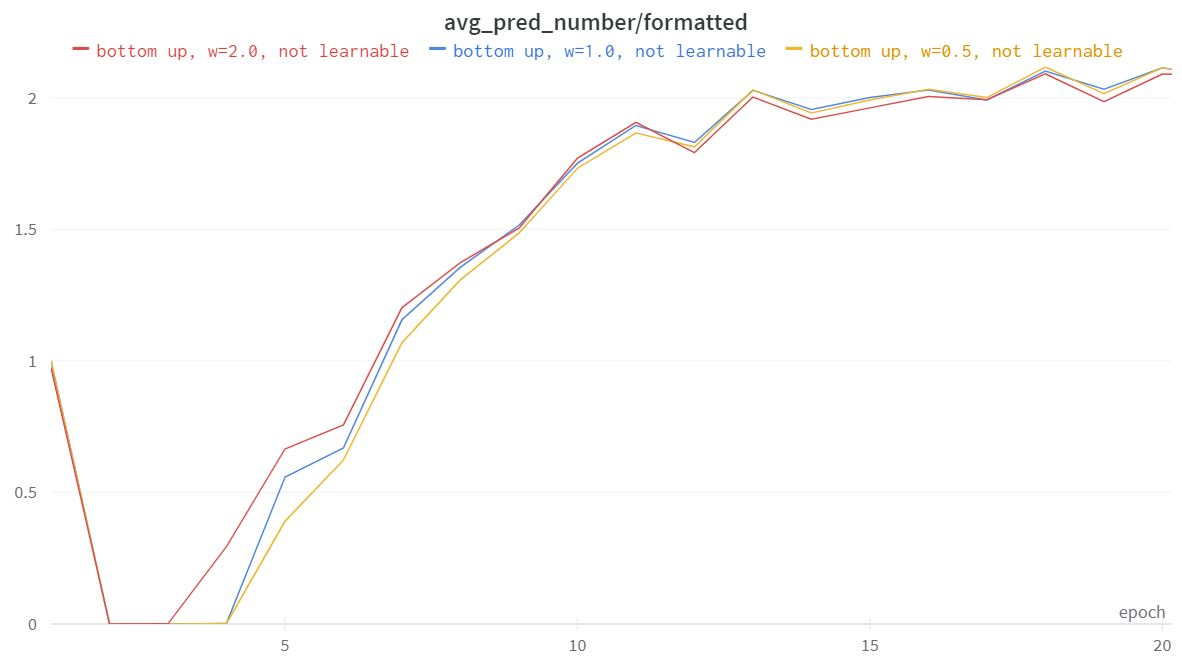
\includegraphics[width=\textwidth]{figures/wandb_weights_bottom_up_avg_pred_start.JPG}
         \caption{Bottom Up}
     \end{subfigure}
     \vfill
     \begin{subfigure}{0.8\textwidth}
         \centering
         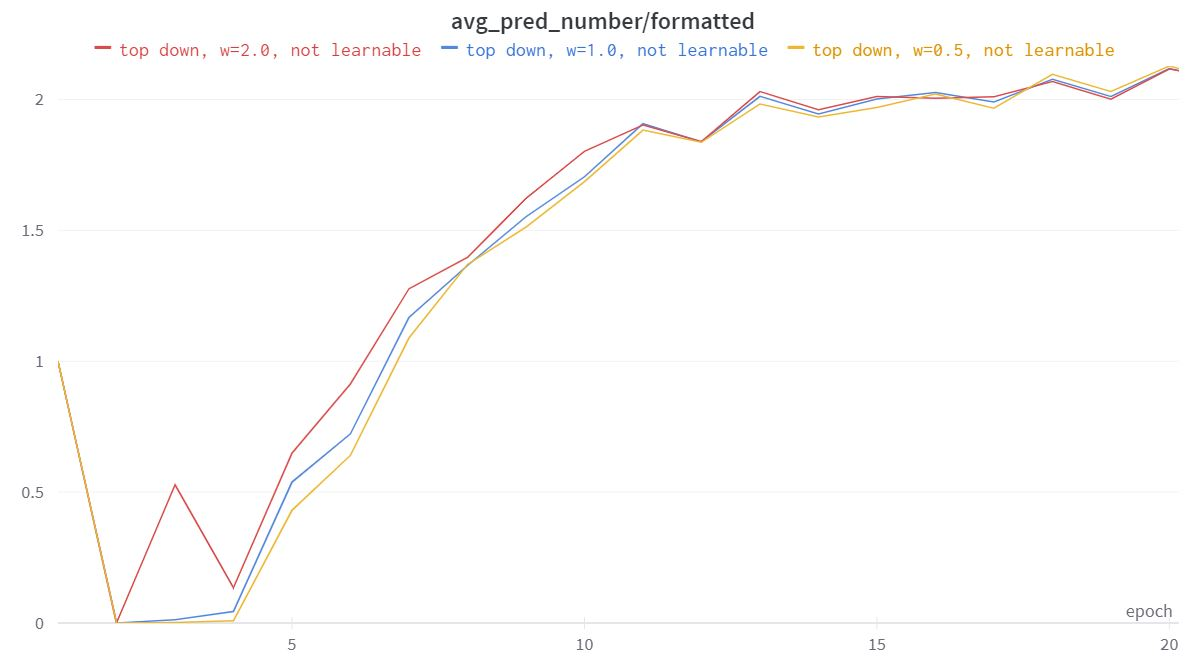
\includegraphics[width=\textwidth]{figures/wandb_weights_top_down_avg_pred_start.JPG}
         \caption{Top Down}
     \end{subfigure}
     \vfill
     \begin{subfigure}{0.8\textwidth}
         \centering
         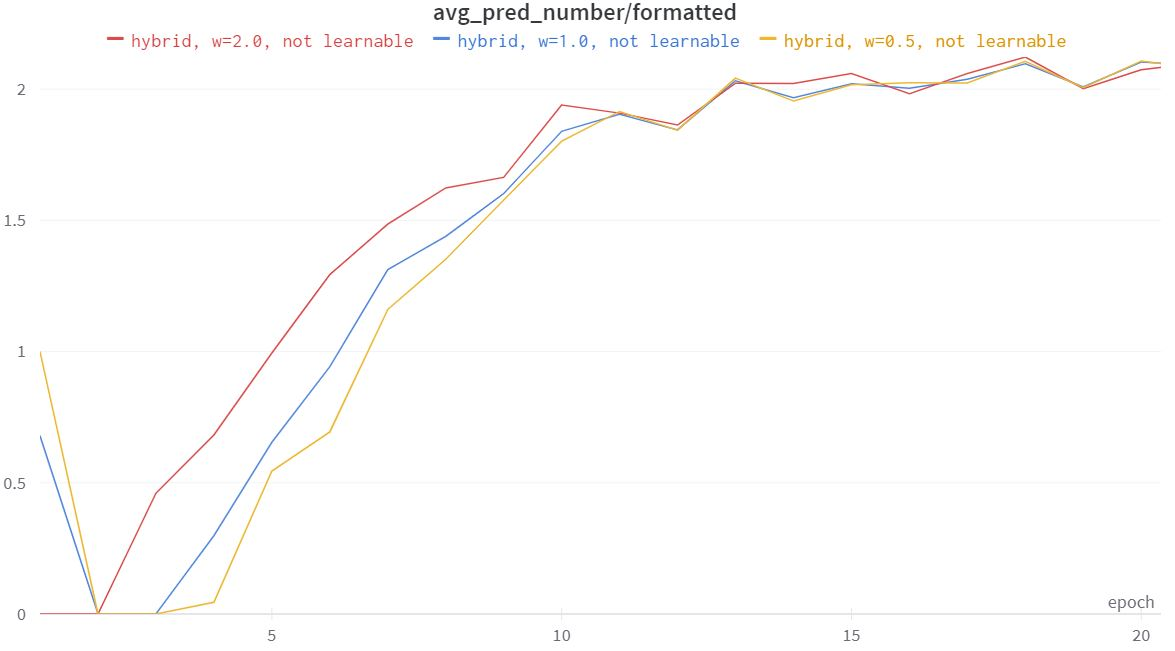
\includegraphics[width=\textwidth]{figures/wandb_weights_hybrid_avg_pred_start.JPG}
         \caption{Hybrid}
     \end{subfigure}
        \caption{Comparison of \textit{average predictions number} by varying the clause weight for each KB mode, with DistilBERT-based models evaluated on the dev set of FIGER. Zoom on the first 20 epochs.}
        \label{fig:wandb_weights_avg_pred_start}
\end{figure}

\paragraphn{Quantitative analysis 2 - KB modes}
Moving on to the comparison between the KB modes, 3 model instances per configuration were trained by varying the random seed. The initial clause weight is set to 2.0 because in the previous experiment was the one that obtained the biggest boost. Figure~\ref{fig:wandb_modes_comparison} reports the comparison graphs in terms of \textit{average predictions number}, \textit{macro f1 examples} and \textit{macro f1 classes }. Similarly to the comparison of the weight, we can draw some considerations about the first steps of the training. Starting from the \textit{average predictions number}, we can clearly observe that the baseline model (i.e, \textit{kb\_mode: - }) produces significantly fewer predictions than KENN in the early stage. In particular, we can notice that the baseline is not able to produce any prediction for the first 4 epochs. Since the pre-KENN network and the baseline network have the same initialization, the fact that KENN requires fewer epochs to make correct predictions is due to the use of logical knowledge.

\begin{figure}[h]
    \centering
    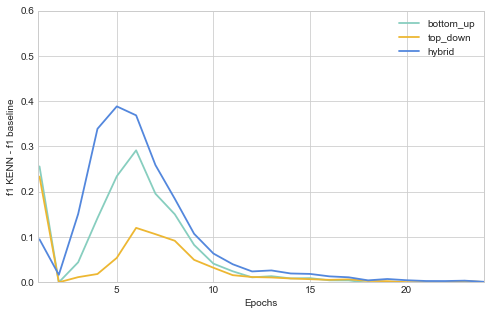
\includegraphics[scale=0.4]{figures/initial_boost.png}
    \caption{Difference between the \textit{macro f1 examples} scores of KENN and baseline models with DistilBERT encoder, evaluated on the dev set of FIGER. The curves are averaged over 3 random seeds. Zoom on the first 25 epochs.}
    \label{fig:initial_boost}
\end{figure}

The trend observed in the \textit{average predictions number} is also detectable by all the other metrics. Figure~\ref{fig:initial_boost} highlights the initial boost of KENN-based models by measuring the difference with respect to the baseline in terms of \textit{macro f1 examples}. The behavior that consolidates as the seeds vary is that Hybrid starts better than Bottom Up, which starts better than Top Down. The baseline model, instead, is the one with the slowest start. The cause of this initial ranking may be that the Hybrid mode can exploit the logical rules of both Bottom Up and Top Down modes. In the second part of the training, instead, the models converge to each other and keep improving together. The results of the final models are reported in Table~\ref{tab:kb_modes_comparison} and are very similar for each KB mode.
% Looking at the graphs in their entirety, there is not a dominant model. However, by looking at the \textit{macro f1 classes} graph we can observe that the baseline model is the only one which never takes the lead.
\begin{figure}
     \centering
     \begin{subfigure}{0.8\textwidth}
         \centering
         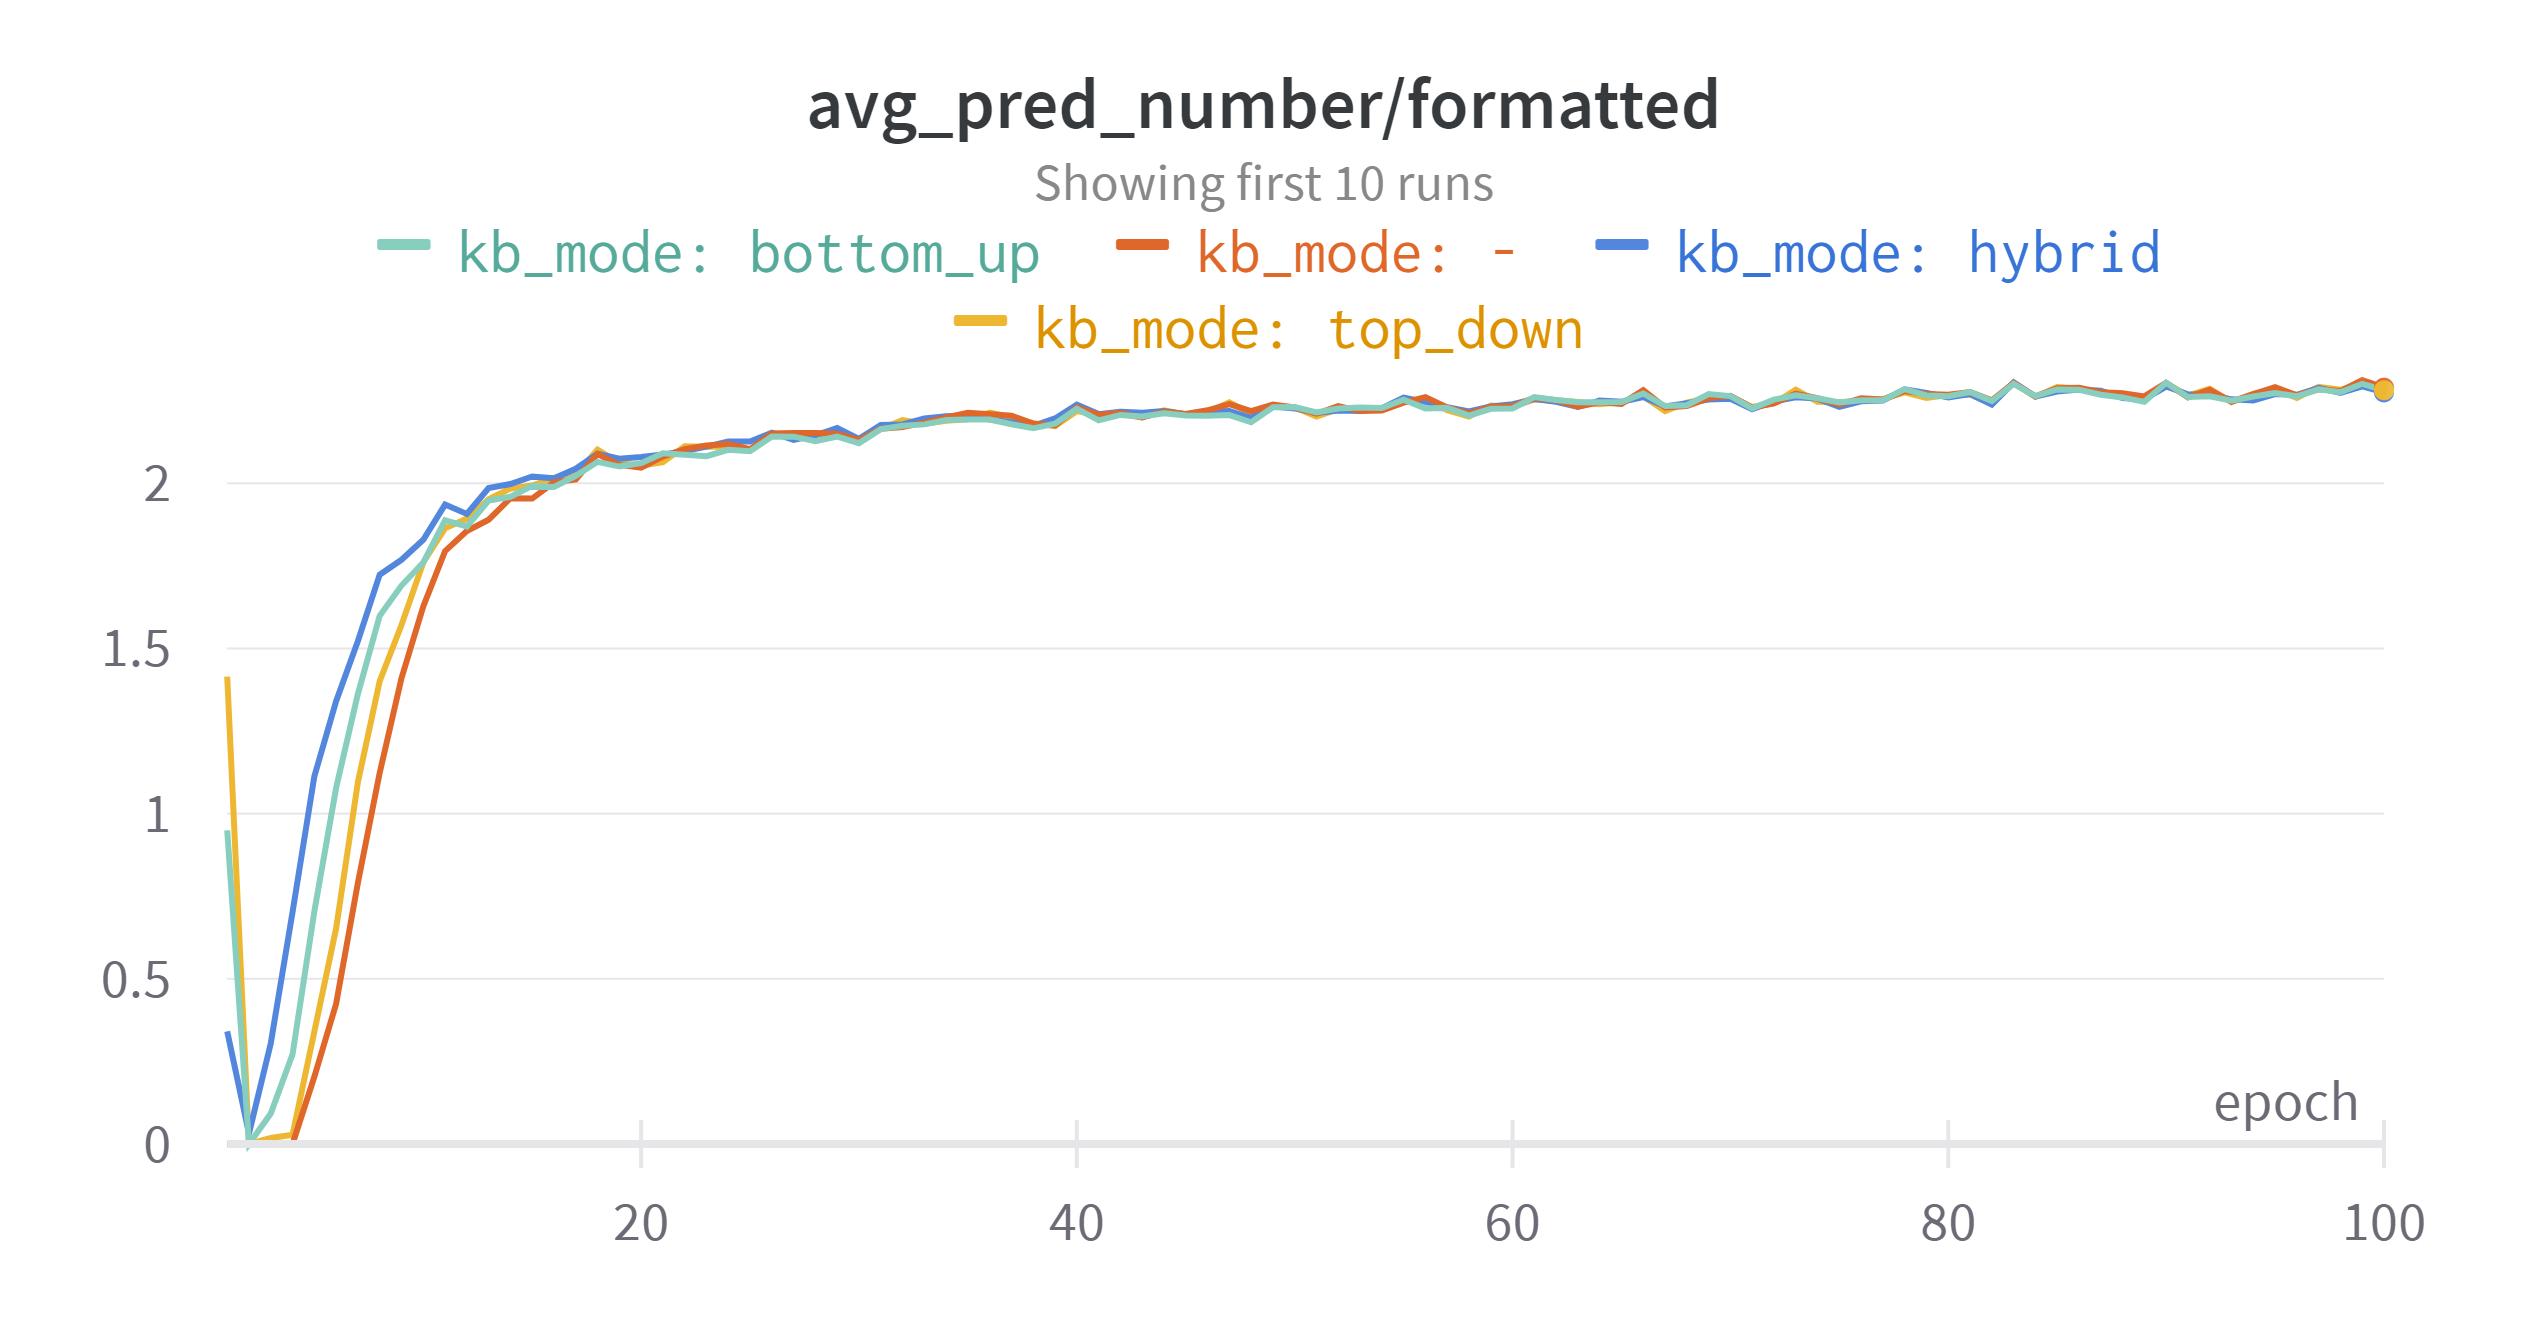
\includegraphics[width=\textwidth]{figures/wandb_modes_avg_pred.png}
         \caption{Average predictions number}
     \end{subfigure}
     \begin{subfigure}{0.8\textwidth}
         \centering
         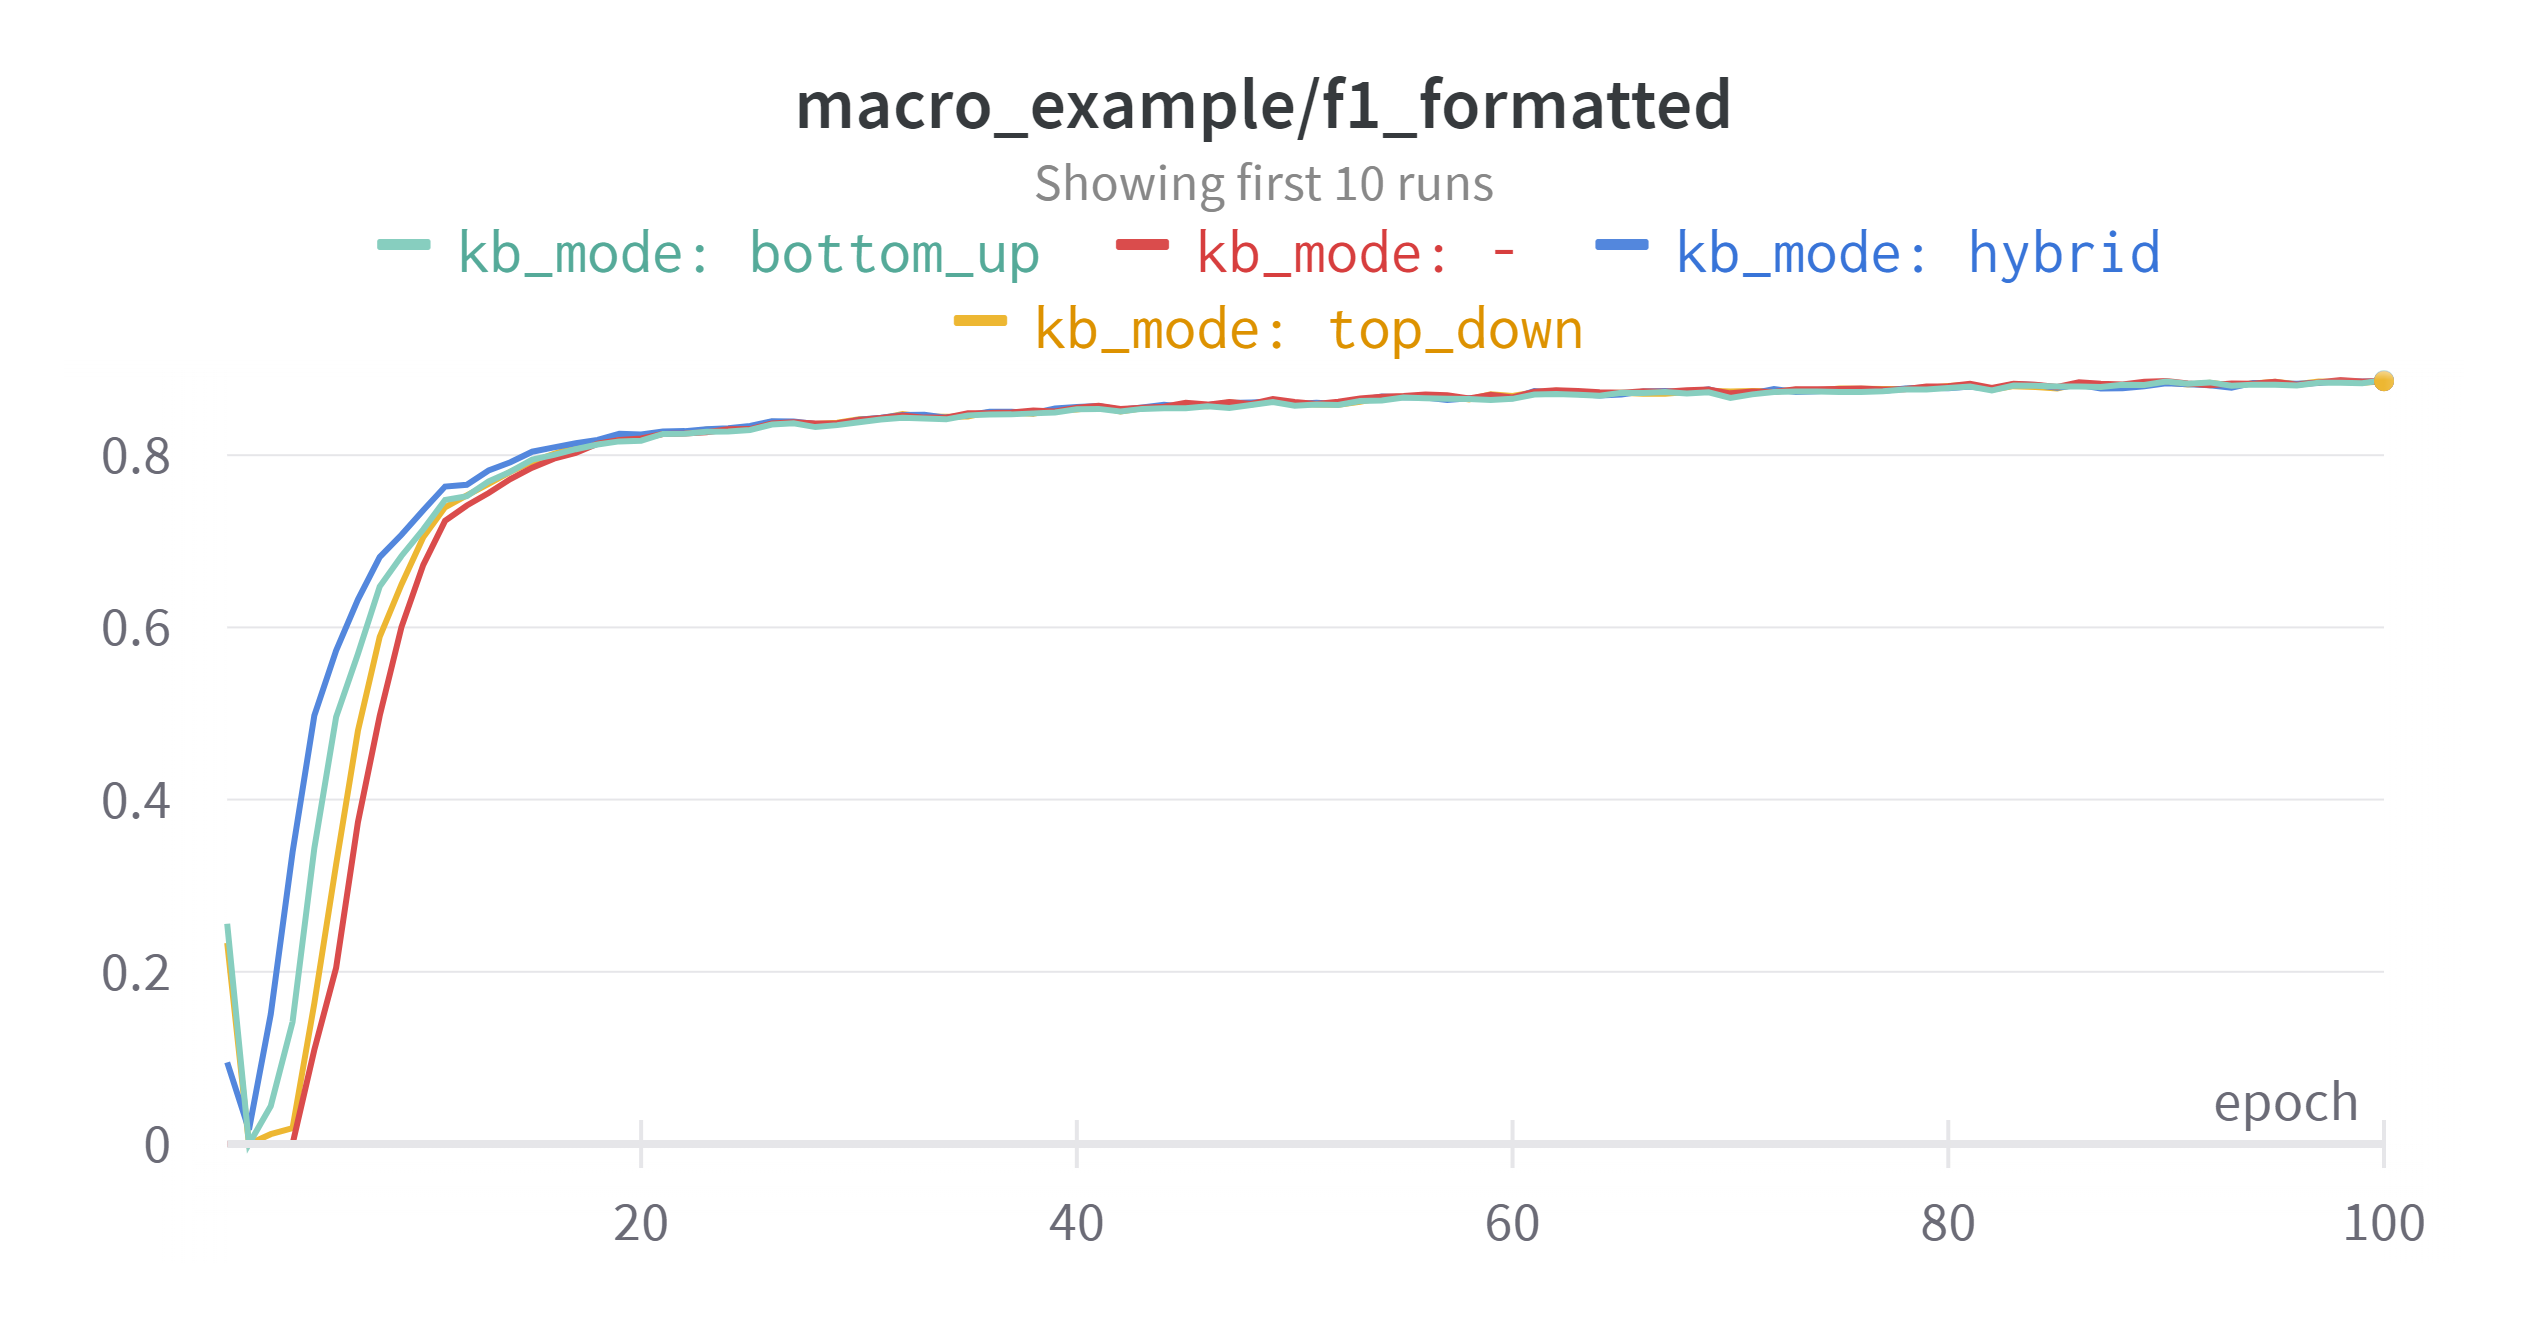
\includegraphics[width=\textwidth]{figures/wandb_modes_macro_ex_f1.png}
         \caption{Macro f1 examples}
     \end{subfigure}
     \begin{subfigure}{0.8\textwidth}
         \centering
         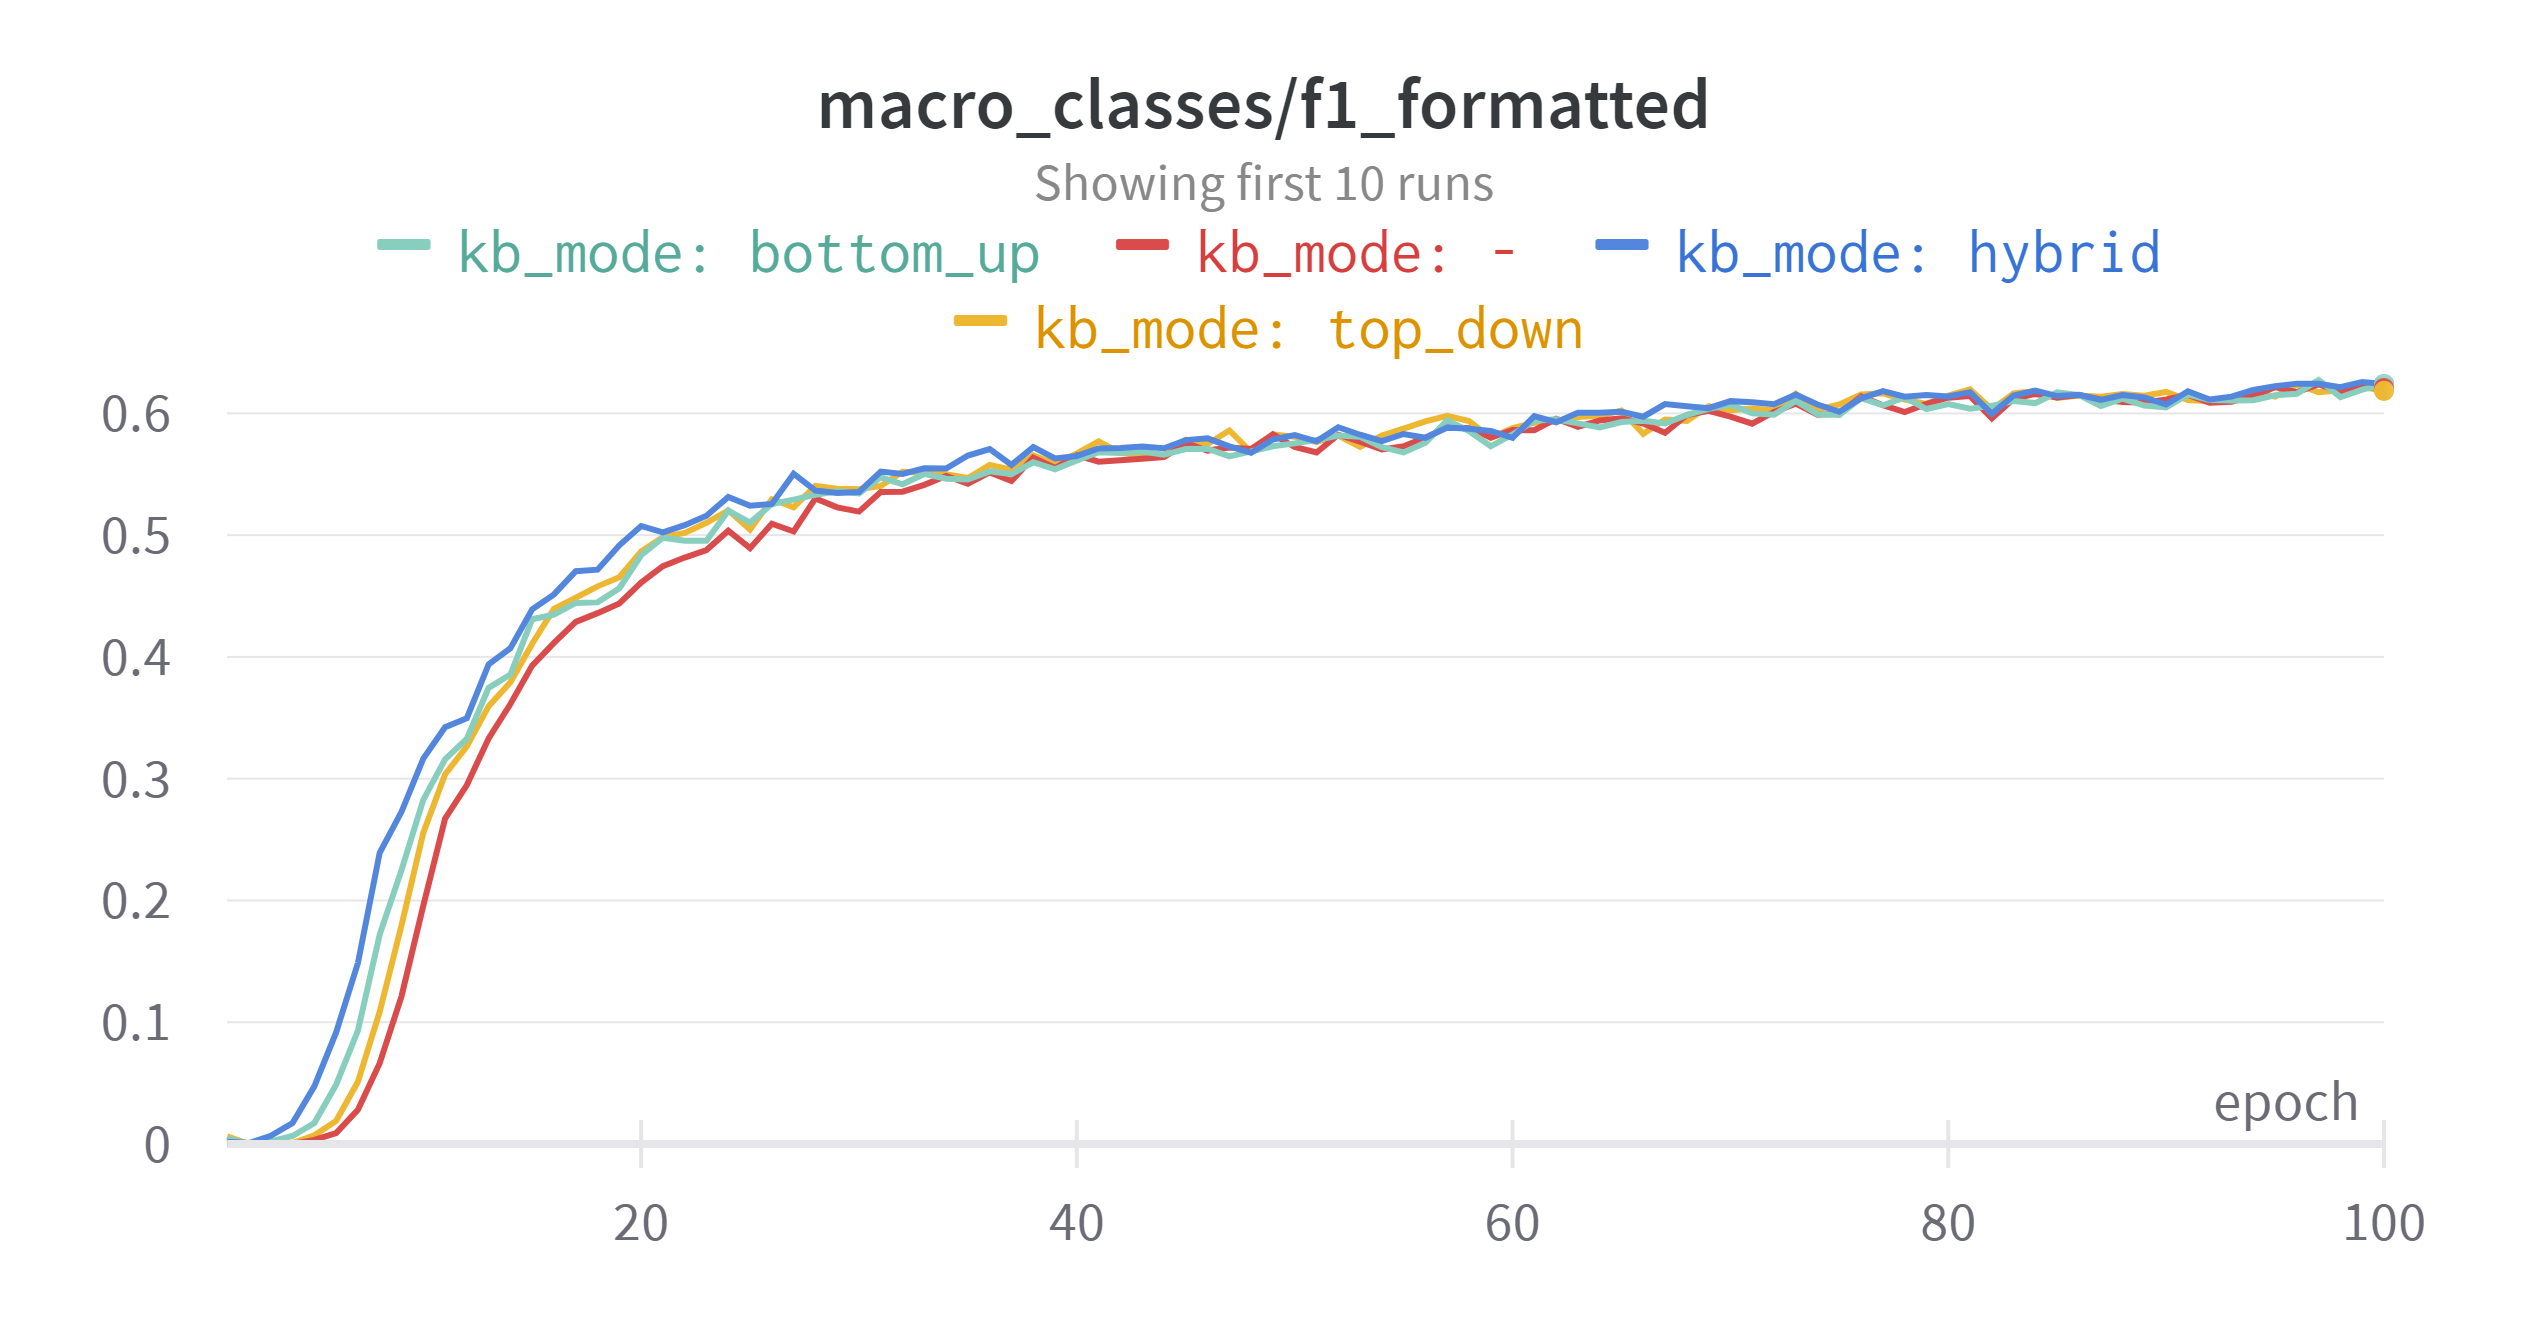
\includegraphics[width=\textwidth]{figures/wandb_modes_macro_class_f1.png}
         \caption{Macro f1 classes}
     \end{subfigure}
        \caption{Comparison between KENN with clause weights fixed to 2.0 and baseline model with DistilBERT encoder, evaluated on the dev set of FIGER. Zoom on the first 20 epochs.}
        \label{fig:wandb_modes_comparison}
\end{figure}

\begin{table}
\centering
\caption{Comparison between KENN with clause weights fixed to 2.0 and baseline model evaluated on the dev set of FIGER. Metrics at epoch 100 averaged over 3 seeds.}
\label{tab:kb_modes_comparison}
\resizebox{\columnwidth}{!}{\begin{tabular}{c|ccc|ccc|}
\cline{2-7}
\textbf{}                            & \multicolumn{3}{c|}{\textbf{Macro examples}}                                                                                                                                                                             & \multicolumn{3}{c|}{\textbf{Macro classes}}                                                                                                                                                                              \\ \hline
\multicolumn{1}{|c|}{\textbf{KB mode}} & \textbf{P}                                                             & \textbf{R}                                                             & \textbf{F1}                                                            & \textbf{P}                                                             & \textbf{R}                                                             & \textbf{F1}                                                            \\ \hline
\multicolumn{1}{|c|}{- (baseline)}       & \begin{tabular}[c]{@{}c@{}}0.8944\\ $\pm$ 0.0009\end{tabular}          & \begin{tabular}[c]{@{}c@{}}0.8779\\ $\pm$ 0.0033\end{tabular}          & \begin{tabular}[c]{@{}c@{}}0.8861\\ $\pm$ 0.0021\end{tabular}          & \begin{tabular}[c]{@{}c@{}}0.6499\\ $\pm$ 0.0152\end{tabular}          & \begin{tabular}[c]{@{}c@{}}0.5943\\ $\pm$ 0.0051\end{tabular}          & \begin{tabular}[c]{@{}c@{}}0.6208\\ $\pm$ 0.0091\end{tabular}          \\ \hline
\multicolumn{1}{|c|}{Bottom Up}      & \begin{tabular}[c]{@{}c@{}}0.8963\\ $\pm$ 0.0.0020\end{tabular}        & \textbf{\begin{tabular}[c]{@{}c@{}}0.8783\\ $\pm$ 0.0047\end{tabular}} & \textbf{\begin{tabular}[c]{@{}c@{}}0.8872\\ $\pm$ 0.0020\end{tabular}} & \begin{tabular}[c]{@{}c@{}}0.6516\\ $\pm$ 0.0165\end{tabular}          & \textbf{\begin{tabular}[c]{@{}c@{}}0.5986\\ $\pm$ 0.0110\end{tabular}} & \begin{tabular}[c]{@{}c@{}}0.6239\\ $\pm$ 0.0115\end{tabular}          \\ \hline
\multicolumn{1}{|c|}{Top Down}       & \begin{tabular}[c]{@{}c@{}}0.8944\\ $\pm$ 0.0008\end{tabular}          & \begin{tabular}[c]{@{}c@{}}0.8777\\ $\pm$ 0.0029\end{tabular}          & \begin{tabular}[c]{@{}c@{}}0.8860\\ $\pm$ 0.0013\end{tabular}          & \begin{tabular}[c]{@{}c@{}}0.6484\\ $\pm$ 0.0088\end{tabular}          & \begin{tabular}[c]{@{}c@{}}0.5913\\ $\pm$ 0.0112\end{tabular}          & \begin{tabular}[c]{@{}c@{}}0.6185\\ $\pm$ 0.0010\end{tabular}          \\ \hline
\multicolumn{1}{|c|}{Hybrid}         & \textbf{\begin{tabular}[c]{@{}c@{}}0.8965\\ $\pm$ 0.0028\end{tabular}} & \begin{tabular}[c]{@{}c@{}}0.8759\\ $\pm$ 0.0025\end{tabular}          & \begin{tabular}[c]{@{}c@{}}0.8861\\ $\pm$ 0.0017\end{tabular}          & \textbf{\begin{tabular}[c]{@{}c@{}}0.6533\\ $\pm$ 0.0185\end{tabular}} & \begin{tabular}[c]{@{}c@{}}0.5974\\ $\pm$ 0.0050\end{tabular}          & \textbf{\begin{tabular}[c]{@{}c@{}}0.6241\\ $\pm$ 0.0112\end{tabular}} \\ \hline
\end{tabular}}
\end{table}

\paragraphn{Quantitative analysis 3 - Metrics per type}
We can observe some interesting behaviors by computing the metrics grouped per types F and S. Focusing on epoch 4 (i.e., the last epoch before the baseline model starts making predictions), it emerges that KENN predicts only types F. This result makes sense since an F type should be easier to predict than an S type, which is more specific. More in detail, Bottom Up and Top Down modes can lead the model to make predictions exclusively on the type \texttt{/location}, reaching an f1 score of 0.595 and 0.441 respectively. The Hybrid model, which achieves an f1 score of 0.747 on \texttt{/location}, can also predict instances of type \texttt{/person} and \texttt{/organization}.

If we now focus on epoch 100, we can observe that Bottom Up performs better than Top Down on types F, with an f1 score of 0.661 and 0.646 respectively. Conversely, if we group the metrics per type S, we can observe that Top Down is better than Bottom Up, with an f1 score of 0.563 and 0.546 respectively. This behavior is consistent with the nature of the different clauses: Bottom Up propagates the information to F, Top Down to S.

\paragraphn{Quantitative analysis - Conclusion}
This analysis points out that the more relevant differences are observable only at the beginning of the training. The initial gap between different clause weights is bridged after 15-20 epochs, as does the difference between the KB modes. The same behavior can be observed when comparing KENN to the baseline model. The suspicion emerging from these considerations is that, at some point of the training, the baseline model becomes as powerful as the KENN-based models. 
%This suspicion can also be extended to the pre-KENN network, which increases its prediction capabilities epoch after epoch, needing less and less KENN's help.
From this premises we can sketch the following hypothesis: the pre-KENN network may adapt its output to obtain some desired predictions after the knowledge enhancement. This hypothesis will be further investigated with the analysis of the preactivations.